\documentclass{article}

% Language setting
% Replace `english' with e.g. `spanish' to change the document language
\usepackage[english]{babel}

% Set page size and margins
% Replace `letterpaper' with `a4paper' for UK/EU standard size
\usepackage[letterpaper,top=2cm,bottom=2cm,left=3cm,right=3cm,marginparwidth=1.75cm]{geometry}

% Useful packages
\usepackage{amsmath}
\usepackage{graphicx}
\usepackage[colorlinks=true, allcolors=blue]{hyperref}

\title{\huge \textbf{A Study of Quantum Imaging}}
\author{Riddhiman Bhattacharya FRSA}

\begin{document}
\maketitle

\begin{abstract}
\large
This article explores quantum optics, where scientists for over two decades have worked on methods to minimize fluctuations in light measurement using quantum techniques. These approaches decrease quantum noise and create strong connections between light particles. Besides focusing on bright light beams, the article emphasizes images formed by light, captured using tools like CCD cameras. Since light adheres to quantum rules, images inevitably encounter unpredictable "quantum noise," complicating reliable information extraction and precise detail spotting. Researchers have worked within the uncertainty principle to control these changes, achieving "spatial quantum entanglement" that links measurements from different image spots. Such techniques promise enhanced image precision, especially valuable in microscopy and data storage. The article concludes with the potential of quantum ideas in image computing, highlighting early-stage research and practical applications.
\end{abstract}

\large



\section{Introduction}
For over twenty years, scientists have developed methods to minimize or lessen wobbles in quantum measurements of light. These methods also create strong quantum links and connections between particles of light. 
Up until now, efforts to reduce quantum noise and enhance correlations have mainly been effective when dealing with the overall brightness of light beams. However, another crucial aspect of optics is the realm of optical images. These images serve as a powerful way to convey a lot of information at once. Devices like CCD cameras or detector arrays, which are made up of tiny elements called pixels, are employed to capture such images. These detectors work whether in situations where individual photons are counted or when dealing with larger groups of photons.

Because light follows quantum rules, the information carried by these images unavoidably experiences unpredictable variations known as "quantum noise" or "shot noise." This noise introduces limitations to how reliably we can extract information from the image or how precisely we can detect small details within it. In the context of these optical measurements, the fluctuations that become important are the local spatial quantum fluctuations.
In the past ten years, researchers have explored theoretical possibilities to shape the small fluctuations in light's spatial properties (within the limits set by \textbf{Heisenberg's uncertainty principle}). They've also demonstrated the ability to create spatial quantum entanglement, which means generating strong quantum connections between measurements taken at different spots on an optical image.

These quantum techniques have the potential to enhance the precision of measurements taken in images and push optical resolution beyond the typical limits defined by the wavelength of light. This applies not only to scenarios where individual photons are counted but also when working with larger beams of light. These innovative techniques could find applications in various fields where light is used for precise physical measurements, like ultraweak absorption spectroscopy or atomic force microscopy. The ability to detect details in images that are smaller than the wavelength is particularly valuable in microscopy, pattern recognition, and optical data storage, where the goal is to store information on areas much tinier than the square of the wavelength.

Moreover, spatial entanglement brings about entirely new and captivating effects. For instance, in two-photon imaging, the camera can be lit up by light that never interacted with the object being imaged. Another example is "\textbf{quantum microlithography}," where quantum entanglement can manipulate matter at a scale smaller than the wavelength.

Looking ahead, there's an exciting possibility to extend quantum information techniques to multimode quantum information and computing using images, although this area is still in its early stages of exploration.
This area of study is a relatively new field within quantum optics, and a handful of pioneering experimental demonstrations have already taken place. The current research primarily focuses on how to create and measure spatially entangled non-classical light, along with initial basic applications that showcase the potential of using these concepts to enhance information retrieval from images.

To make these somewhat abstract ideas clearer, we'll now provide a brief overview of a few accomplishments in this domain. We'll conclude by mentioning some potential directions and challenges that hold promise and warrant further investigation in the future. \footnote{For further studies refer this \cite{kolobov1999}}

\section{The Quantum Laser Pointer}

In experiments, researchers have observed that when performing precise optical measurements on the overall brightness or phase of a light beam, they can improve sensitivity by using special types of light known as \textbf{sub-Poissonian} or \textbf{squeezed states}. This method works effectively when analyzing the entire light beam as a whole. However, when the goal is to measure changes in the distribution of light across an optical image, the same approach isn't applicable.

For instance, consider the measurement of the center position of a light beam using a quadrant detector (\ref{f-1}). If the partial intensities received by the four segments are equal, it indicates that the beam is accurately centered on the detector. Any imbalance in the received intensities provides information about the transverse displacement of the beam. This measurement is highly sensitive and can reach scales as small as nanometers. Nevertheless, like other optical measurements, it is limited by standard quantum noise, often referred to as shot noise, which affects the four segments of the quadrant detector.

Theoretically, it was demonstrated for the first time by Fabre \cite{Fabre:00} that it's possible to surpass this standard quantum limit and enhance pointing sensitivity. This can be achieved by using a unique combination of light—a single-mode squeezed beam combined with a coherent beam, where the two halves of the beam are shifted by $\pi$ relative to each other in the transverse plane. This peculiar mixture generates a perfect quantum correlation between the intensities measured on the two halves of the combined beam. As a result, this correlation affects the photocurrents detected on the corresponding pixels of the detector.


\begin{figure}
    \centering
    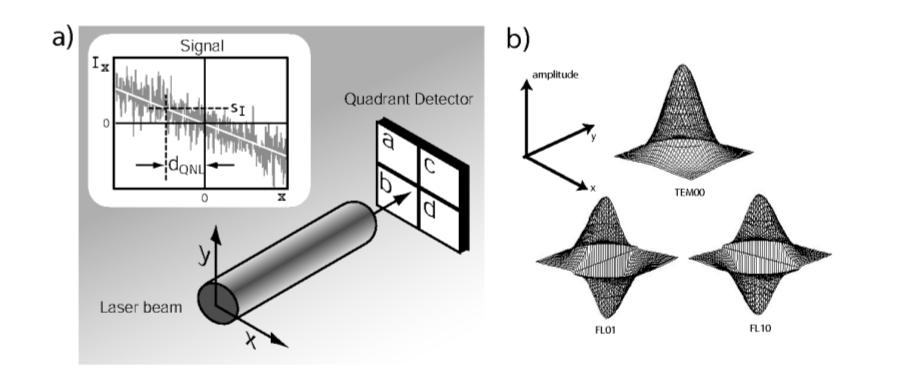
\includegraphics[width=0.7\textwidth]{Fig 1.jpeg}
    \caption{Caption}
    \label{f-1}
\end{figure}
This phenomenon has recently been shown through experiments \cite{doi:10.1126/science.1086489}. The beam's central displacements in two directions were measured with greater sensitivity than what's conventionally achievable in quantum systems. To simultaneously gauge both transverse coordinates with precision surpassing shot noise limitations, a three-mode nonclassical light state is required. This state is a combination of two squeezed states and a coherent state, with each transverse mode having specific $\pi$ phase shifts in the four quadrants of the transverse plane, corresponding to the four regions of detection. The simplest multi-pixel detector measurement involves transverse displacement, yet an image can yield various other parameters. These include detecting the motion of a tiny scattering object, a faint spatial modulation, or the presence of digitized information in small holes (like those in CDs used for optical data storage). Extracting such information relies on "image processing," which generally entails calculating linear combinations of local intensities captured by different pixels. This issue has been extensively explored theoretically \cite{PhysRevA.71.013820}. For any linear processing, the transverse mode contributing to noise in this form of image processing has been identified. By decreasing noise in this specific mode, the accuracy of corresponding information determination is enhanced. This technique holds promise for enhancing functions like pattern recognition, image segmentation, and wavefront analysis in image processing and analysis.

On the quantum information front, recent theoretical proposals have emerged for generating spatially entangled beams \cite{Hsu_2005}. These beams extend the transverse measurement problem associated with the entangled state originally suggested by Einstein, Podolsky, and Rosen \cite{PhysRev.47.777} for X and P measurements. In these "EPR-entangled beams," measurements of transverse position x for two light beams show perfect correlation, while measurements of angular tilt $\theta$ with respect to the optical axis exhibit perfect anti-correlation. In the transverse plane, x and $\theta$ represent quantum-conjugate quantities, akin to X and P for a particle.

\section{Control and Utilization of Quantum Noise in Spatial Domain.}
The experiment discussed in the previous section demonstrates the ability to control the transverse arrangement of temporal quantum fluctuations in light. However, within an image, there exists what can be called "pure" spatial quantum noise. This refers to the fluctuations in light intensity from pixel to pixel when integrated over the entire duration of a single light pulse. It exclusively pertains to spatial averages and doesn't involve time averages.

Measuring these pixel-to-pixel fluctuations at the quantum level presents a new and demanding experimental challenge. Innovative and intricate experimental techniques had to be developed to attain the shot noise level for spatial fluctuations. A crucial step involves highly precise calibration of each pixel on the detector to ensure that the measured intensity on each pixel can be correctly normalized \cite{refId0}. Only after resolving all these technical issues was it feasible to observe the two distinct spatial quantum phenomena described in the subsequent subsections.

\subsection{Detection and Study of Pure Spatial Quantum Correlations in Parametric
Down Conversion}
It's widely recognized that parametric down conversion generates "twin photons" \cite{neves2005generation} that exhibit perfect quantum-level correlation. This correlation is not only temporal (the photons are generated simultaneously) but also spatial (they emerge in symmetric directions). This phenomenon has been extensively utilized in remarkable milestone experiments involving photon counting. When the pump intensity is significantly increased, numerous twin photons are generated, and they can no longer be individually enumerated. Instead, patterns or "images" appear on the signal and idler beams. These images maintain temporal and spatial quantum-level correlation. As shown in Figure \ref{fig:2}, each image displays significant fluctuations from pixel to pixel, yet the intensity values on pixels symmetrically positioned relative to the figure's center are nearly identical.
\begin{figure}
    \centering
    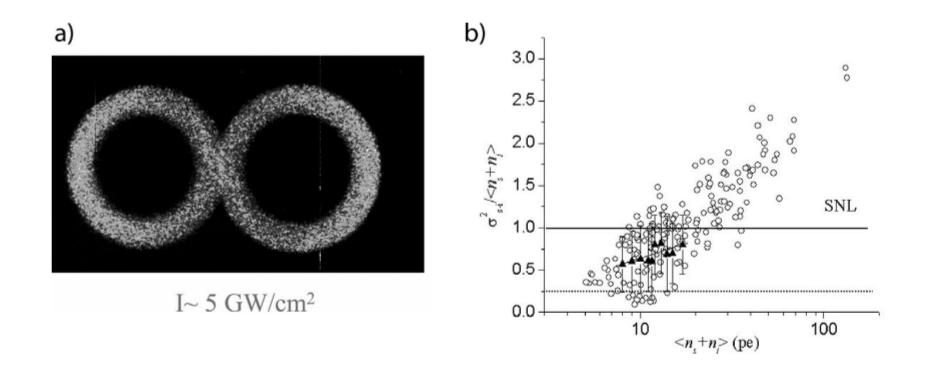
\includegraphics[width=0.7\textwidth]{Fig 2.jpeg}
    \caption{a) When spontaneous parametric down-conversion is driven by very high intensities I, causing numerous photons to simultaneously converge on the same point, light is emitted.\\
b) The difference in intensity noise between two symmetric pixels, averaged over all pixels, changes with the gain as a result of high pump intensities. The horizontal solid line represents the standard quantum limit.}
    \label{fig:2}
\end{figure}

The experiment \cite{PhysRevLett.93.243601} employed an intense pulse laser to drive the spontaneous down-conversion process. Operating in such a regime yielded a high parametric gain (ranging from 10 to 1000), and approximately 10 to 100 photons were recorded on average per pixel. Notably, a pixel-to-pixel quantum correlation emerged between the intensity patterns of the signal and idler transverse distributions after a single pulse from the pump laser.

To elaborate, the variance of the intensity disparity between the signal and idler modes, measured on symmetrical pixels and averaged across various points in the transverse plane, was found to be well below the standard quantum limit. In this case, the limit corresponds to the spatial shot noise derived from the total intensities measured on the photodetectors. The most significant reduction in spatial noise observed was approximately $50\%$ below the standard quantum limit.

Interestingly, when the gain is set very high, the quantum correlation eventually diminishes. This transition from the quantum to the classical realm arises due to the increased gain causing the signal or idler beams generated by the nonlinear crystal to narrow spatially. This narrowing leads to a diffraction-induced expansion of the region where the twin photons are distributed. The observed quantum spatial correlation now offers the potential to enhance information processing in images. For instance, it could be used to increase the sensitivity for detecting faint images below the standard quantum limit.
\subsection{Optical Amplification}
\textbf{Optical amplification} stands as a pivotal technique in the realm of optical information manipulation. Within quantum theory, it's evident that the amplification process unavoidably introduces a minimum degradation of the signal-to-noise ratio by a factor of 2. This degradation transpires when oscillating signals are amplified without regard to the phase of oscillation. However, in contrast, amplification can be achieved without noise increase in the phase-sensitive configuration.

Parametric amplification, especially in the frequency degenerate setup, can indeed operate in such a phase-sensitive manner. Consequently, it can amplify an optical signal while preserving its quality.

This distinctive trait of degenerate parametric amplifiers was established through demonstrations involving the total intensities of amplified signal beams in pulsed parametric amplifiers. This property also extends to image amplification. The experimental proof of noiseless image amplification marked the first instance of validating a quantum imaging phenomenon. 
\begin{figure}[h]
    \centering
    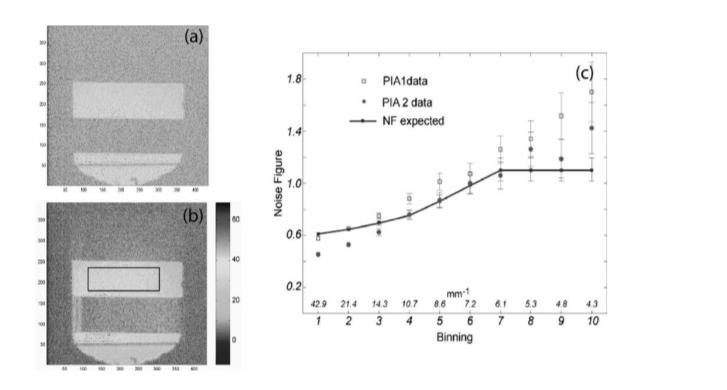
\includegraphics[width=0.7\textwidth]{Fig 3.jpeg}
    \caption{a) Image without amplification, (b) amplified image in a phase insensitive ampli-
fier, and (c) effective noise figure (ratio between the noises of the amplified and nonamplified
image divided by the gain) versus the number of neighboring pixels used to determine the noise}
    \label{hi}
\end{figure}

This phenomenon was observed in the temporal fluctuations recorded across different points of an image \cite{PhysRevLett.83.1938}. Moreover, the phenomenon was recently validated for the intrinsic pixel-to-pixel spatial fluctuations of an image amplified through a pulsed optical parametric amplifier and captured in a single shot using a pump laser \cite{article}. In a meticulously designed experiment, spatial noise characteristics were evaluated in both phase-sensitive and phase-insensitive configurations. Notably, in the low-gain regime, the phase-sensitive amplifier did not introduce noise, while the phase-insensitive amplifier led to a 2-fold degradation of the signal-to-noise ratio [Fig \ref{hi}]. 

The prospect of amplifying faint images without compromising their quality holds significant promise for various applications.

\section{Two-Photon Imaging}
Two-photon imaging, often referred to as "ghost imaging," is a captivating phenomenon rooted in the spatial correlations of light. The initial demonstration of this effect was achieved by exploiting the spatial quantum correlations present between the signal and idler twin photons generated through spontaneous parametric down-conversion \cite{PhysRevLett.74.3600}. Here's how it works [fig \ref{fig:4}]
\begin{figure}[h]
    \centering
    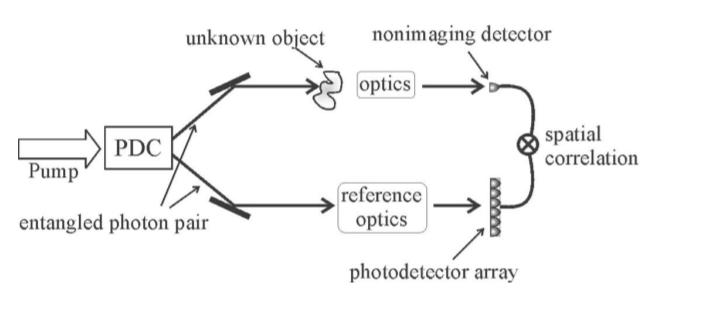
\includegraphics[width=0.7\textwidth]{Fig 4.jpeg}
    \caption{Two-photon Imaging}
    \label{fig:4}
\end{figure}

In the signal arm, an object intended for observation is introduced. Surprisingly, the image of this object is acquired without utilizing a pixelated detector. Instead, a nonimaging "bucket" detector is employed on the signal beam, which measures only the total intensity that passes through the object. Simultaneously, in the idler arm, a pixelated detector (like a CCD camera) is placed where there's no object. The object's image is reconstructed by retaining information from the CCD camera only when its measurement coincides with a photon detection by the "bucket" detector. This technique was executed at the level of photon counting in several elegant experiments during the mid-1990s. It was widely regarded as a prime example of leveraging spatial quantum correlations in the photon-counting realm.

Subsequently, it was demonstrated that the same imaging setup could be used to observe the effect even with the intense light produced in the high-gain regime of parametric amplification. Specifically, the image emerges from the correlation between the total intensity of the signal beam and the spatially resolved intensity distribution of the idler beam. Additionally, it was predicted that both the image itself (often referred to as the "near-field image") and its Fourier transform (which can be obtained, for instance, through diffraction in the far-field regime, known as the \textbf{far-field image}) could be determined using the same experimental configuration. Given that these two quantities bear some resemblance to conjugate variables like position and momentum, this property was deemed connected to the EPR (Einstein-Podolsky-Rosen) nature of the spatial correlation between the signal and idler beams.

In a recent experimental study \cite{PhysRevLett.92.069901}, it was demonstrated that a near-field image could be generated using the same technique by employing classically correlated beams derived from a beam-splitter, rather than using twin photons. This discovery ignited a lively global debate surrounding the accurate categorization of classical and quantum attributes in the context of "two-photon imaging." Notably, it was found and experimentally validated \cite{PhysRevLett.93.093602} that the identical imaging method could yield both near-field and far-field images using a thermal beam divided into two parts via a beam-splitter, rather than employing quantum-correlated beams. When opting for quantum-correlated beams instead of classical correlations, certain quantitative aspects, such as image contrast, exhibit improvement. From an application standpoint, the fact that enigmatic "ghost imaging" can be achieved through a simple beam-splitter and a thermal light source, as opposed to using twin beams generated by a complex setup, is advantageous in terms of cost and simplicity. This underscores the practical significance of accurately differentiating between classical and quantum aspects within a given phenomenon, a discourse that is often perceived as purely theoretical.

\section{Other Prospective Areas in Quantum Imaging}

Within the realm of quantum imaging, one specific area of inquiry holds significant importance—research into the quantum limitations on optical resolution. This field bears the potential to introduce novel concepts in microscopy and optical data storage. "Super-resolution techniques" have long been explored within classical contexts, aiming to surpass the Rayleigh limit of resolution, which is typically on the order of the wavelength. In theory, deconvolution techniques could potentially extract the shape of a very small object from its image, even if diffraction has caused significant blurring. However, the presence of noise in the image, including quantum noise, ultimately hampers such a flawless reconstruction process. Noise serves to curtail the amount of information that can be extracted regarding the shape of the small object.

This process of object reconstruction has recently been revisited from a quantum perspective \cite{PhysRevLett.85.3789}. It has been demonstrated that, in principle, the performance of super-resolution techniques could be improved by introducing nonclassical light into specific transverse modes, specifically the eigenmodes governing propagation through the imaging system. The exact method for generating such multi-mode nonclassical light has also been determined. The simplicity of the proposed approach instills confidence that quantum-enhanced super-resolution techniques can be effectively implemented in practical experiments.
Transverse solitons hold promise as potential candidates for spatial qubits, while soliton arrays could serve as q-registers. Recent theoretical exploration has focused on their quantum attributes in various setups. This includes solitons that propagate freely through planar Kerr media \cite{EricLantz_2004} and cavity solitons that emerge in degenerate parametric oscillators \cite{Oppo2007}. As a preliminary step towards investigating quantum information processing, these devices have been predicted to exhibit local noise reduction and spatial correlations.

Nonlinear media have long been used for image processing. For instance, up-conversion of optical images from the infrared to the visible spectrum has been proposed and realized, aiming to leverage the superior quality of CCD detectors in the visible range. This domain has also seen recent exploration in the context of quantum-level investigation through second harmonic generation. Certain configurations have been identified where up-converting any image to the second harmonic field is possible without introducing quantum noise to the initial image.

Furthermore, it's intriguing to consider how established "classical" protocols in quantum information, such as teleportation or cryptography, could be extended to the realm of images. This exploration involves understanding how the inherent parallelism inherent in imaging could be harnessed within these protocols. Quantum teleportation of images has been a particularly detailed subject of study \cite{IvanVSokolov_2001}. The proposed scheme shares many similarities with conventional holographic techniques, but with the notable advantage that, in the quantum teleportation scheme, the image reproduction process doesn't introduce additional quantum noise.

\section{Conclusion and Perspectives}
Microscopy, wavefront correction, image processing, optical data storage, and general optical measurements constitute a crucial realm within today's technologies. These fields can derive various advantages from the ongoing research in quantum imaging, an area that is currently being explored by an increasing number of research teams worldwide.
While optical technologies could directly benefit from the advancements achieved through quantum effects demonstrated in laboratory experiments, their present complexity poses a challenge to immediate practical applications. Taking a more practical and feasible approach, many optical technologies could experience substantial enhancements by employing the advanced techniques developed in quantum optics labs to achieve and surpass the threshold of quantum noise in images.
Significant research efforts are still required, both on the experimental front to enhance light sources and detectors for achieving high levels of quantum spatial entanglement, and on the theoretical front to discover more practical applications of spatial entanglement in information technologies. A promising avenue of exploration lies in leveraging the orbital angular momentum of light to transmit and process quantum information. So far, spatial quantum effects have primarily been applied in the fields of metrology and information storage, residing somewhat on the periphery of quantum computing. There have been no proposals to exploit the parallelism of optical imaging within quantum computing algorithms. While undoubtedly challenging, this area is undeniably captivating. It necessitates collaborative efforts between the quantum computing and quantum imaging communities.
\newpage
\bibliographystyle{unsrt}
\bibliography{references}
\end{document}






